
%使用xelatex编译
%版权所有,翻版必究
%本文件由程序自动生成,任何修改将被覆盖
%2019 年 01 月 09 日





\FloatBarrier
\section{
你好世界!
}\label{s100410}




\begin{figure}[ht] %浮动体 here and top ...
\centering %中心对齐
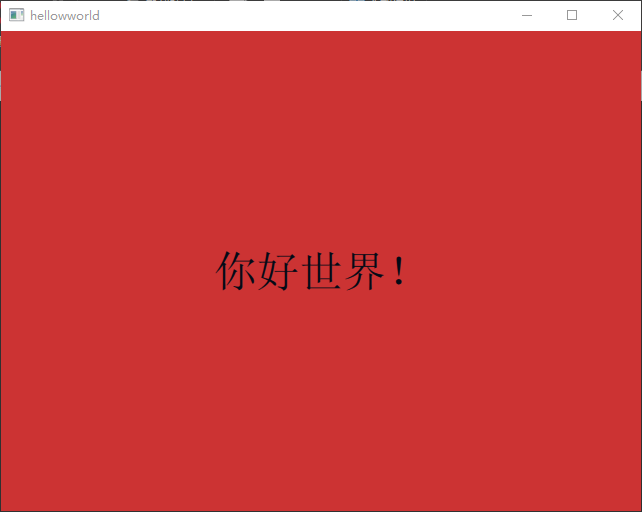
\includegraphics[width=0.95\textwidth]{../chapter01/hellowworld/the_app.png} %图片路径
\caption{你好世界!} %标题
\label{p000006} %索引
\end{figure}




%\begin{spacing}{1.0}
\begin{lstlisting}[label=f000030,
caption=GoodLuck,
title=\lstlistingname\ \thelstlisting
]
#include <sstd_qt_and_qml_library.hpp>

int main(int argc, char ** argv) {

    /*初始化程序*/
    auto varApp = sstd_make_unique< sstd::Application >(argc, argv);
    /*初始化Qml/Quick引擎*/
    auto varWindow = sstd_make_unique< sstd::DefaultRoowWindow >();
    {
        /*获得Qml文件绝对路径*/
        auto varFullFileName = sstd::getLocalFileFullPath(
            QStringLiteral("myqml/hellowworld/main.qml"));
        /*加载Qml文件*/
        varWindow->load(varFullFileName);
        /*检查并报错*/
        if (varWindow->status() != sstd::LoadState::Ready) {
            qWarning() << QStringLiteral("can not load : ") << varFullFileName;
            return -1;
        }
    }
    varWindow->show();

    return varApp->exec();

}
\end{lstlisting}          %抄录环境
%\end{spacing}
%main.cpp
%\begin{spacing}{1.0}
\begin{lstlisting}[label=f000031,
caption=GoodLuck,
title=\lstlistingname\ \thelstlisting
]
/*main.qml*/
import QtQuick 2.9
import "main_private" as MainPrivate

Rectangle {

    width: 640
    height: 480
    color: Qt.rgba(0.8, 0.8, 0.8, 1)

    MainPrivate.MainText {
        z: 1
        anchors.fill: parent
    } /*~MainText*/

    MainPrivate.MainRectangle {
        z: 0
        anchors.fill: parent
    } /*~MainRectangle*/
} /*~Rectangle*/
\end{lstlisting}          %抄录环境
%\end{spacing}
%main.qml
%\begin{spacing}{1.0}
\begin{lstlisting}[label=f000032,
caption=GoodLuck,
title=\lstlistingname\ \thelstlisting
]
/*main_private/MainRectangle.qml*/
import QtQuick 2.9

Rectangle {
    color: Qt.rgba(0.8, 0.2, 0.2, 1)
}
\end{lstlisting}          %抄录环境
%\end{spacing}
%MainRectangle.qml
%\begin{spacing}{1.0}
\begin{lstlisting}[label=f000033,
caption=GoodLuck,
title=\lstlistingname\ \thelstlisting
]
/*main_private/MainText.qml*/
import QtQuick 2.9

Text {
    text: qsTr("你好世界!")
    color: Qt.rgba(Math.random() / 10, Math.random() / 10,
                   Math.random() / 10, 1)
    font.pointSize: 32
    verticalAlignment: Text.AlignVCenter
    horizontalAlignment: Text.AlignHCenter
}
\end{lstlisting}          %抄录环境
%\end{spacing}
%MainText.qml







%使用xelatex编译
%版权所有,翻版必究
%本文件由程序自动生成,任何修改将被覆盖
%2019 年 01 月 09 日



